\documentclass[tikz,border=4pt]{standalone}
\usepackage[T1]{fontenc}
\usepackage{amsmath}
\usepackage[scaled=0.96]{helvet}
\renewcommand{\familydefault}{\sfdefault}
\usepackage{xcolor}
\usetikzlibrary{arrows.meta,calc}

\definecolor{Ink}{HTML}{3B3B3B}
\definecolor{Accent}{HTML}{B00300}
\definecolor{Arrow}{HTML}{5F5F5F}
\definecolor{Border}{HTML}{CFC3B3}
\definecolor{PanelBg}{HTML}{EFE2D0}
\definecolor{CardBg}{HTML}{FCDEB9}
\definecolor{Zero}{HTML}{FCDEB9}
\definecolor{One}{HTML}{3B3B3B}
\definecolor{OrbitA}{HTML}{FCDEB9}
\definecolor{OrbitB}{HTML}{EFE2D0}
\definecolor{OrbitC}{HTML}{E2E2E2}
\definecolor{OrbitD}{HTML}{F3D5D0}
\definecolor{WinnerBg}{HTML}{FCDEB9}

\tikzset{
  panel title/.style={anchor=west,text=Ink,font=\bfseries\fontsize{11.5}{11.5}\selectfont},
  panel sub/.style={text=Ink,align=center,text width=3.75cm,font=\fontsize{8.4}{9.7}\selectfont},
  panel foot/.style={text=Ink,align=center,text width=4.05cm,font=\fontsize{8.0}{9.1}\selectfont},
  soft frame/.style={draw=black!20,line width=0.7pt},
  row box/.style={draw=black!18,fill=CardBg,line width=0.6pt,rounded corners=2.0pt},
  score box/.style={draw=black!18,fill=CardBg,line width=0.6pt,rounded corners=2.0pt},
  winner box/.style={draw=Arrow!55!black,fill=WinnerBg,line width=0.8pt,rounded corners=2.0pt}
}

\newcommand{\DrawBinaryGrid}[3]{%
  \fill[Zero] (#1,#2) rectangle ++(1.8,1.35);
  \foreach \c/\r in {#3}{
    \fill[One] ({#1 + 0.225*\c},{#2 + 1.35 - 0.225*(\r+1)}) rectangle ++(0.225,0.225);
  }
  \draw[draw=black!35, line width=0.45pt] (#1,#2) rectangle ++(1.8,1.35);
  \foreach \i in {1,...,7} {
    \draw[draw=black!35, line width=0.45pt] ({#1 + 0.225*\i},#2) -- ({#1 + 0.225*\i},{#2 + 1.35});
  }
  \foreach \j in {1,...,5} {
    \draw[draw=black!35, line width=0.45pt] (#1,{#2 + 0.225*\j}) -- ({#1 + 1.8},{#2 + 0.225*\j});
  }
}

\newcommand{\DrawSmallBinaryGrid}[3]{%
  \fill[Zero] (#1,#2) rectangle ++(0.82,0.82);
  \foreach \c/\r in {#3}{
    \fill[One] ({#1 + 0.205*\c},{#2 + 0.82 - 0.205*(\r+1)}) rectangle ++(0.205,0.205);
  }
  \draw[draw=black!35, line width=0.45pt] (#1,#2) rectangle ++(0.82,0.82);
  \foreach \i in {1,...,3} {
    \draw[draw=black!35, line width=0.45pt] ({#1 + 0.205*\i},#2) -- ({#1 + 0.205*\i},{#2 + 0.82});
    \draw[draw=black!35, line width=0.45pt] (#1,{#2 + 0.205*\i}) -- ({#1 + 0.82},{#2 + 0.205*\i});
  }
}

\newcommand{\Panel}[3]{%
  \begin{scope}[shift={(#1,0)}]
    \fill[PanelBg] (0,0) rectangle (4.8,5.95);
    \draw[draw=Border, line width=0.8pt] (0,0) rectangle (4.8,5.95);
    \fill[Accent] (0.38,5.69) circle[radius=0.20];
    \node[text=PanelBg, font=\bfseries\small] at (0.38,5.69) {#2};
    \node[panel title] at (0.96,5.67) {#3};
  \end{scope}
}

\newcommand{\VoteRow}[6]{%
  \draw[row box] (#1,#2) rectangle ++(3.28,0.56);
  \fill[#4] ({#1 + 0.14},{#2 + 0.10}) rectangle ++(0.42,0.36);
  \draw[draw=black!22, line width=0.4pt] ({#1 + 0.14},{#2 + 0.10}) rectangle ++(0.42,0.36);
  \node[text=black!70, font=\bfseries\fontsize{8.6}{8.6}\selectfont] at ({#1 + 0.35},{#2 + 0.28}) {#3};
  \node[text=Ink, font=\fontsize{9.2}{9.2}\selectfont] at ({#1 + 1.55},{#2 + 0.28}) {#5};
  \draw[draw=Arrow!80!black, line width=0.95pt, -{Latex[length=2.6mm,width=2.2mm]}] ({#1 + 2.28},{#2 + 0.28}) -- ({#1 + 2.72},{#2 + 0.28});
  \fill[#6] ({#1 + 2.82},{#2 + 0.12}) rectangle ++(0.32,0.32);
  \draw[draw=black!28, line width=0.45pt] ({#1 + 2.82},{#2 + 0.12}) rectangle ++(0.32,0.32);
}

\begin{document}
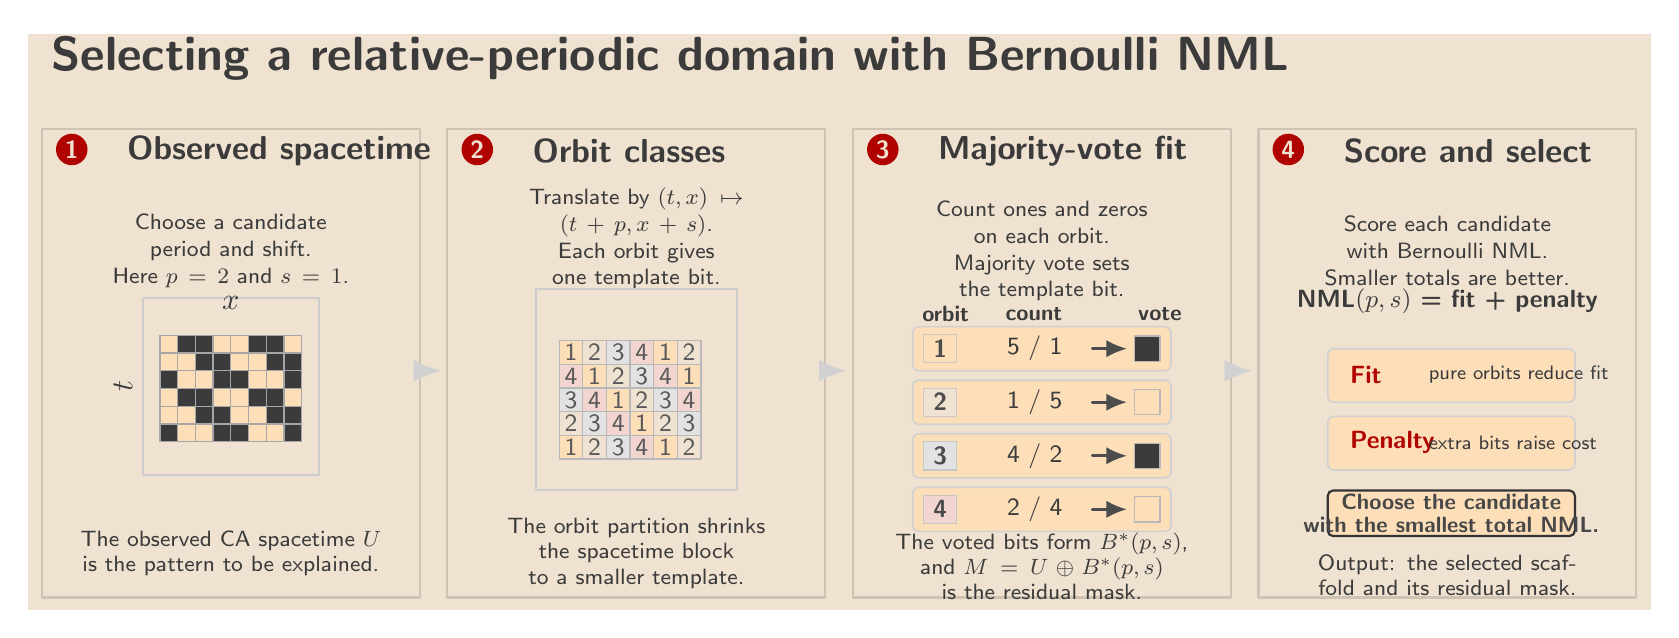
\begin{tikzpicture}[x=1cm,y=1cm,>=Latex,line cap=round,line join=round]
  \fill[PanelBg] (-0.18,-0.16) rectangle (20.43,7.16);
  \node[anchor=west, text=Ink, font=\bfseries\fontsize{17}{19}\selectfont] at (0,6.85) {Selecting a relative-periodic domain with Bernoulli NML};

  \Panel{0.0}{1}{Observed spacetime}
  \Panel{5.15}{2}{Orbit classes}
  \Panel{10.30}{3}{Majority-vote fit}
  \Panel{15.45}{4}{Score and select}

  \draw[draw=black!18, fill=black!18, line width=1.0pt, -{Latex[length=3.5mm,width=2.8mm]}] (4.87,2.88) -- (5.07,2.88);
  \draw[draw=black!18, fill=black!18, line width=1.0pt, -{Latex[length=3.5mm,width=2.8mm]}] (10.02,2.88) -- (10.22,2.88);
  \draw[draw=black!18, fill=black!18, line width=1.0pt, -{Latex[length=3.5mm,width=2.8mm]}] (15.17,2.88) -- (15.37,2.88);

  % Panel 1
  \begin{scope}[shift={(0,0)}]
    \node[panel sub] at (2.40,4.40) {Choose a candidate\\period and shift.\\Here $p=2$ and $s=1$.};
    \draw[soft frame] (1.28,1.56) rectangle (3.52,3.80);
    \node[text=Ink, font=\fontsize{10.5}{10.5}\selectfont] at (2.40,3.74) {$x$};
    \node[text=Ink, font=\fontsize{10.5}{10.5}\selectfont, rotate=90] at (1.03,2.68) {$t$};
    \DrawBinaryGrid{1.50}{1.98}{1/0,2/0,5/0,6/0,2/1,3/1,6/1,7/1,0/2,3/2,4/2,7/2,1/3,2/3,5/3,6/3,2/4,3/4,6/4,7/4,0/5,3/5,4/5,7/5}
    \node[panel foot] at (2.40,0.56) {The observed CA spacetime $U$ is the pattern to be explained.};
  \end{scope}

  % Panel 2
  \begin{scope}[shift={(5.15,0)}]
    \node[panel sub] at (2.40,4.56) {Translate by $(t,x)\mapsto$\\$(t+p,x+s)$.\\Each orbit gives one template bit.};
    \draw[soft frame] (1.12,1.36) rectangle (3.68,3.92);
    \foreach \c/\r/\lab/\col in {0/0/1/OrbitA,1/0/2/OrbitB,2/0/3/OrbitC,3/0/4/OrbitD,4/0/1/OrbitA,5/0/2/OrbitB,0/1/4/OrbitD,1/1/1/OrbitA,2/1/2/OrbitB,3/1/3/OrbitC,4/1/4/OrbitD,5/1/1/OrbitA,0/2/3/OrbitC,1/2/4/OrbitD,2/2/1/OrbitA,3/2/2/OrbitB,4/2/3/OrbitC,5/2/4/OrbitD,0/3/2/OrbitB,1/3/3/OrbitC,2/3/4/OrbitD,3/3/1/OrbitA,4/3/2/OrbitB,5/3/3/OrbitC,0/4/1/OrbitA,1/4/2/OrbitB,2/4/3/OrbitC,3/4/4/OrbitD,4/4/1/OrbitA,5/4/2/OrbitB} {
      \fill[\col] ({1.42 + 0.30*\c},{1.76 + 1.50 - 0.30*(\r+1)}) rectangle ++(0.30,0.30);
      \draw[draw=black!28, line width=0.45pt] ({1.42 + 0.30*\c},{1.76 + 1.50 - 0.30*(\r+1)}) rectangle ++(0.30,0.30);
      \node[text=black!65, font=\fontsize{8.8}{8.8}\selectfont] at ({1.42 + 0.30*\c + 0.15},{1.76 + 1.50 - 0.30*(\r+1) + 0.15}) {\lab};
    }
    \node[panel foot] at (2.40,0.56) {The orbit partition shrinks the spacetime block to a smaller template.};
  \end{scope}

  % Panel 3
  \begin{scope}[shift={(10.30,0)}]
    \node[panel sub] at (2.40,4.40) {Count ones and zeros\\on each orbit.\\Majority vote sets the template bit.};
    \node[text=Ink, font=\bfseries\fontsize{8.3}{8.3}\selectfont] at (1.18,3.60) {orbit};
    \node[text=Ink, font=\bfseries\fontsize{8.3}{8.3}\selectfont] at (2.30,3.60) {count};
    \node[text=Ink, font=\bfseries\fontsize{8.3}{8.3}\selectfont] at (3.90,3.60) {vote};
    \VoteRow{0.76}{2.88}{1}{OrbitA}{5 / 1}{One}
    \VoteRow{0.76}{2.20}{2}{OrbitB}{1 / 5}{Zero}
    \VoteRow{0.76}{1.52}{3}{OrbitC}{4 / 2}{One}
    \VoteRow{0.76}{0.84}{4}{OrbitD}{2 / 4}{Zero}
    \node[panel foot] at (2.40,0.40) {The voted bits form $B^*(p,s)$, and $M = U \oplus B^*(p,s)$ is the residual mask.};
  \end{scope}

  % Panel 4
  \begin{scope}[shift={(15.45,0)}]
    \node[panel sub] at (2.40,4.40) {Score each candidate\\with Bernoulli NML.\\Smaller totals are better.};
    \node[text=Ink, font=\bfseries\fontsize{9.0}{9.0}\selectfont] at (2.40,3.76) {NML$(p,s)$ = fit + penalty};
    \draw[score box] (0.88,2.48) rectangle (4.02,3.16);
    \node[anchor=west, text=Accent, font=\bfseries\fontsize{8.6}{8.6}\selectfont] at (1.04,2.83) {Fit};
    \node[anchor=west, text=Ink, font=\fontsize{7.4}{8.2}\selectfont] at (2.04,2.83) {pure orbits reduce fit};
    \draw[score box] (0.88,1.62) rectangle (4.02,2.30);
    \node[anchor=west, text=Accent, font=\bfseries\fontsize{8.6}{8.6}\selectfont] at (1.04,1.97) {Penalty};
    \node[anchor=west, text=Ink, font=\fontsize{7.4}{8.2}\selectfont] at (2.04,1.97) {extra bits raise cost};
    \draw[winner box] (0.88,0.78) rectangle (4.02,1.36);
    \node[text=Arrow!75!black, align=center, font=\bfseries\fontsize{7.7}{8.3}\selectfont] at (2.45,1.07) {Choose the candidate\\with the smallest total NML.};
    \node[panel foot] at (2.40,0.28) {Output: the selected scaffold and its residual mask.};
  \end{scope}
\end{tikzpicture}
\end{document}
